%-------------------------------------------%
\newpage
\section{Stability Margins}
%-------------------------------------------%
When designing a control system,  the first thing we want to ensure is the \textbf{stability} of the closed-loop system.

\begin{itemize}
    \item Stability margins measure how close the system is to instability: less margin, less stable
    
    \item There are 2 ways to make the system unstable:
    \begin{itemize}
        \item \textbf{Increase controller gain}, this reduces the \textbf{gain margin}.
        \item \textbf{Increase time delay}, this reduces the \textbf{phase margin}.
    \end{itemize}
    \begin{figure}[H] 
        \centering
        % 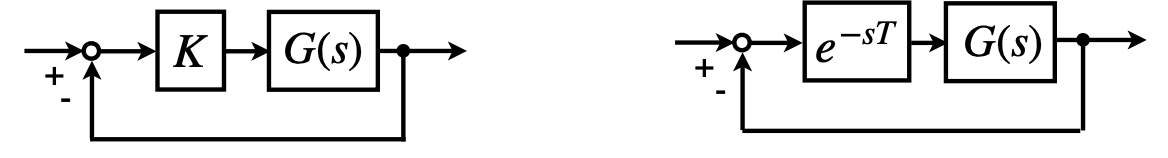
\includegraphics[width=0.75\textwidth]{images/unstable.png}
        \begin{tikzpicture}[auto, node distance=2cm,>=latex',line width=1pt, scale=0.45]
    \node [input, name=input] {};
    \node [sum, right of=input] (sum) {};
    \node [block, right of=sum] (controller1) {$K$};
    \node [block, right= 1cm of controller1] (controller2) {$G(s)$};
    \coordinate [right=1cm of controller2, circle, scale=0.5, fill](tooutput){};
    \node [output, right=1cm of tooutput] (output) {};
    \coordinate [below= 1.5cm of tooutput] (measurements) {};

    \draw [draw,->] (input) -- node {$U(s)$\ {\footnotesize$+$}} (sum); 
    \draw [->] (sum) -- node {} (controller1);
    \draw [->] (controller1) -- (controller2);
    \draw [-] (controller2) -- (tooutput);
    \draw [->] (tooutput) -- node[] {$Y(s)$} (output);
    \draw [-] (tooutput) |- (measurements);
    \draw [->] (measurements) -| 
    node[pos=1] {{\footnotesize$-$}} (sum);
\end{tikzpicture}
\quad
\begin{tikzpicture}[auto, node distance=2cm,>=latex',line width=1pt, scale=0.45]
    \node [input, name=input] {};
    \node [sum, right of=input] (sum) {};
    \node [block, right of=sum] (controller1) {$e^{-sT}$};
    \node [block, right= 1cm of controller1] (controller2) {$G(s)$};
    \coordinate [right=1cm of controller2, circle, scale=0.5, fill](tooutput){};
    \node [output, right=1cm of tooutput] (output) {};
    \coordinate [below= 1.5cm of tooutput] (measurements) {};

    \draw [draw,->] (input) -- node {$U(s)$\ {\footnotesize$+$}} (sum); 
    \draw [->] (sum) -- node {} (controller1);
    \draw [->] (controller1) -- (controller2);
    \draw [-] (controller2) -- (tooutput);
    \draw [->] (tooutput) -- node[] {$Y(s)$} (output);
    \draw [-] (tooutput) |- (measurements);
    \draw [->] (measurements) -| 
    node[pos=1] {{\footnotesize$-$}} (sum);
\end{tikzpicture}
        \caption{Two ways to make the system unstable}
    \end{figure}

    \item Two closed-loop, feedback systems have same characteristic functions. The open-loop transfer function, $C(s)H(s)$, determines the stability of the closed-loop systems:
    \begin{figure}[H] 
        \centering
        % 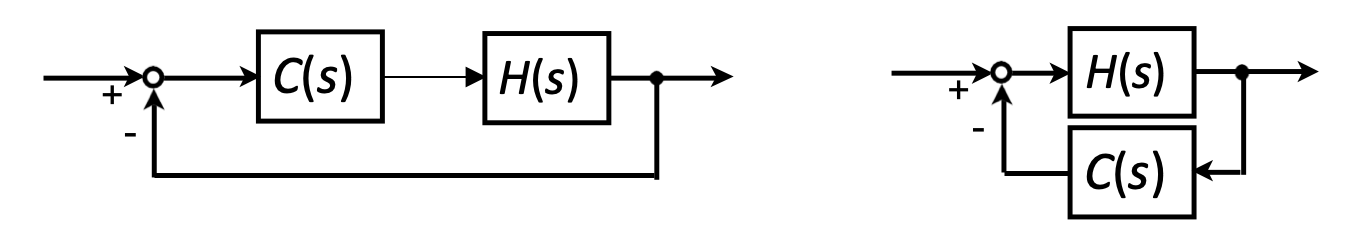
\includegraphics[width=0.65\textwidth]{images/closed_loop_stability.png}
        \begin{tikzpicture}[auto, node distance=2cm,>=latex',line width=1pt]
    \node [input, name=input] {};
    \node [sum, right of=input] (sum) {};
    \node [block, right of=sum] (controller1) {$C(s)$};
    \node [block, right= 1cm of controller1] (controller2) {$H(s)$};
    \coordinate [right=1cm of controller2](tooutput){};
    \node [output, right=1cm of tooutput] (output) {};
    \coordinate [below= 1cm of tooutput] (measurements) {};

    \draw [draw,->] (input) -- node {$U(s)$\ {\footnotesize$+$}} (sum); 
    \draw [->] (sum) -- node {} (controller1);
    \draw [->] (controller1) -- (controller2);
    \draw [-] (controller2) -- (tooutput);
    \draw [->] (tooutput) -- node[] {$Y(s)$} (output);
    \draw [-] (tooutput) |- (measurements);
    \draw [->] (measurements) -| 
    node[pos=1] {{\footnotesize$-$}} (sum);
\end{tikzpicture}

\begin{tikzpicture}[auto, node distance=2cm,>=latex',line width=1pt]
    \node [input, name=input] {};
    \node [sum, right of=input] (sum) {};
    \node [block, right of=sum] (controller1) {$H(s)$};
    \node [block, below= 0.5cm of controller1] (controller2) {$C(s)$};
    \coordinate [right=1cm of controller1](tooutput){};
    \node [output, right=1cm of tooutput] (output) {};

    \draw [draw,->] (input) -- node {$U(s)$\ {\footnotesize$+$}} (sum); 
    \draw [->] (sum) -- node {} (controller1);
    \draw [-] (controller1) -- (tooutput);
    \draw [-] (controller1) -- (tooutput) |- (controller2) ;
    \draw [->] (controller2) -| node[pos=1] {{\footnotesize$-$}} (sum);
    \draw [->] (tooutput) -- node[] {$Y(s)$} (output);
\end{tikzpicture}
    \end{figure} 
    
    \vspace{-1cm}
    \[
    G(s) = \frac{C(s)H(s)}{1+C(s)H(s)} \quad \quad \quad G(s) =\frac{H(s)}{1+C(s)H(s)} 
    \]\\
    The closed-loop system becomes unstable if the gain of the closed loop system is $\infty$. Specifically, in this case, denominator $\to 0$:
    \[
    1+C(s)H(s) =0 \quad \leftrightarrow  \quad \underbrace{C(s)H(s)}_{\text{open-loop transfer function}}=-1 \quad \leftrightarrow \quad \begin{cases}
    \lvert C(s)H(s) \rvert =1 \\
    \angle C(s)H(s) =-180^{\circ}\\
    \end{cases} 
    \]
    
    \item To make the Bode plot of $G_{D}(s) = C(s)H(s)$:
        \begin{figure}[H] 
            \centering
            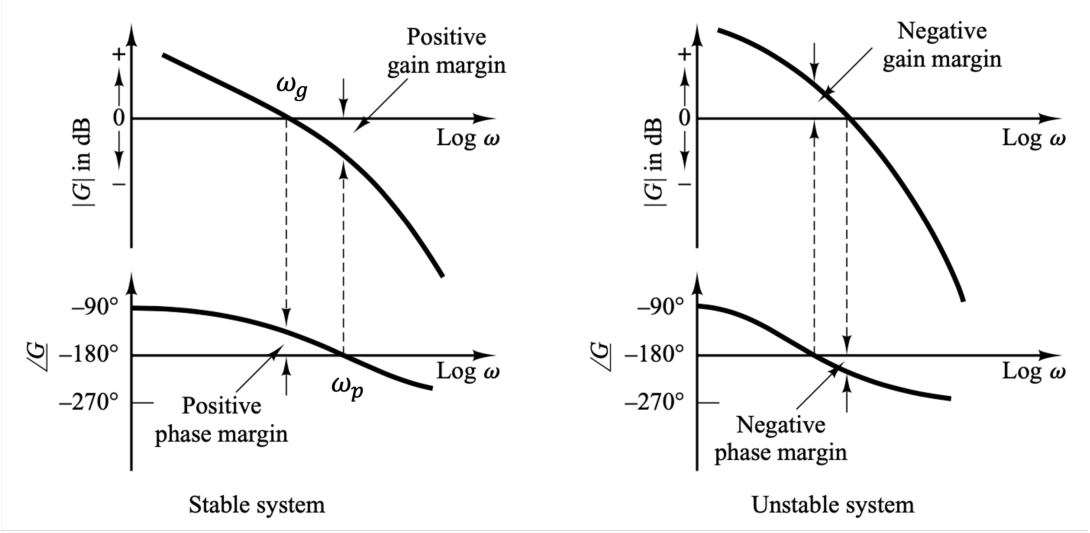
\includegraphics[width=0.85\textwidth]{images/margin.pdf}
            \caption{Stability margins for stable and unstable systems}
        \end{figure}
        
    \begin{itemize}
        \item Stability margin for stable systems: before losing the stability, we can 
        \begin{enumerate}
            \item add the same amount of \underline{phase delay} as the \textbf{positive phase margin}, at $\omega$, where $\lvert G(\omega)\rvert=0dB$
            \item add the same amount of \underline{gain} as the \textbf{positive phase margin}, at $\omega$, where $\angle G(\omega)=-180^{\circ}$
        \end{enumerate}
    
        \item Stability margin for unstable systems: the system can become stable if we 
            \begin{enumerate}
                \item reduce the same amount of \underline{phase delay} as the \textbf{negative phase margin}, at $\omega$, where $\lvert G(\omega)\rvert=0dB$
                \item reduce the same amount of \underline{gain} as the \textbf{negative gain margin}, at $\omega$, where $\angle G(\omega)=-180^{\circ}$
            \end{enumerate}
    \end{itemize}
\end{itemize}

%-------------------------------------------%
\subsection{Gain margin}
%-------------------------------------------%
The gain margin is the gain relative to $0dB$ when $\angle G(j\omega_{p}) = -180^{\circ}$:
 \[ GM = -20\log_{10}\lvert G(j\omega_{p})\rvert\]
 \ where $\omega_{p}$ is known as \textbf{phase cross-over frequency}, $\angle G(j\omega_{p}) = -180^{\circ}$. 

%-------------------------------------------%
\subsection{Phase margin}
%-------------------------------------------%
The \textbf{phase margin} is the phase relative to $180^{\circ}$ when $\lvert G(j\omega_{g}) \rvert =1$:
\[ PM = \angle G(j\omega_{g})-(-180^{\circ}) =\angle G(j\omega_{g})+ 180^{\circ}\] 
\ where $\omega_{g}$ is known as the \textbf{gain cross-over frequency}, $20\log \lvert G(j\omega_{g})\rvert = 0$.

%-------------------------------------------%
\subsection{Delay margin}
%-------------------------------------------%
Delay margin is the translation of phase margin in the delay time.
\[T = \frac{PM}{\omega_{g}}\frac{\pi}{180^{\circ}}\]
The system becomes unstable when the open-loop transfer function satisfies $e^{sT}G(s) = -1$ at the gain cross-over frequency, $\omega_{g}$.
\begin{align*}
\begin{split}
e^{-j\omega_{g}T}G(j\omega_{g})=-1
\quad \longrightarrow \quad 
 \angle (e^{j\omega_{g}T} G(j\omega_{g}))&= \angle (e^{j\omega_{g}T})+\angle G(j\omega_{g}) \\
&= -\omega_{g}T\cdot \frac{180^{\circ}}{\pi}+PM-180^{\circ} \\
&= -180^{\circ}
\end{split}
\end{align*}

%-------------------------------------------%
\newpage
\section{State-space Representation}
%-------------------------------------------%
\begin{itemize}
  \item \textbf{State-space representation} is a convenient way to describe \textbf{multi-input/multi-output} LTI systems in time domain using matrix algebra.
  
  \item The system is described as a set of inputs, $\mathbf{u}(t)$, outputs, $\mathbf{y}(t)$, and state variables, $\mathbf{x}(t)$.
  \begin{itemize}
    \item \textbf{State variables} is a set of variables that uniquely determines the current condition of the system (\textit{e.g.} position, temperature, protein concentration)
 \end{itemize}

    \begin{figure}[H] 
        \centering
        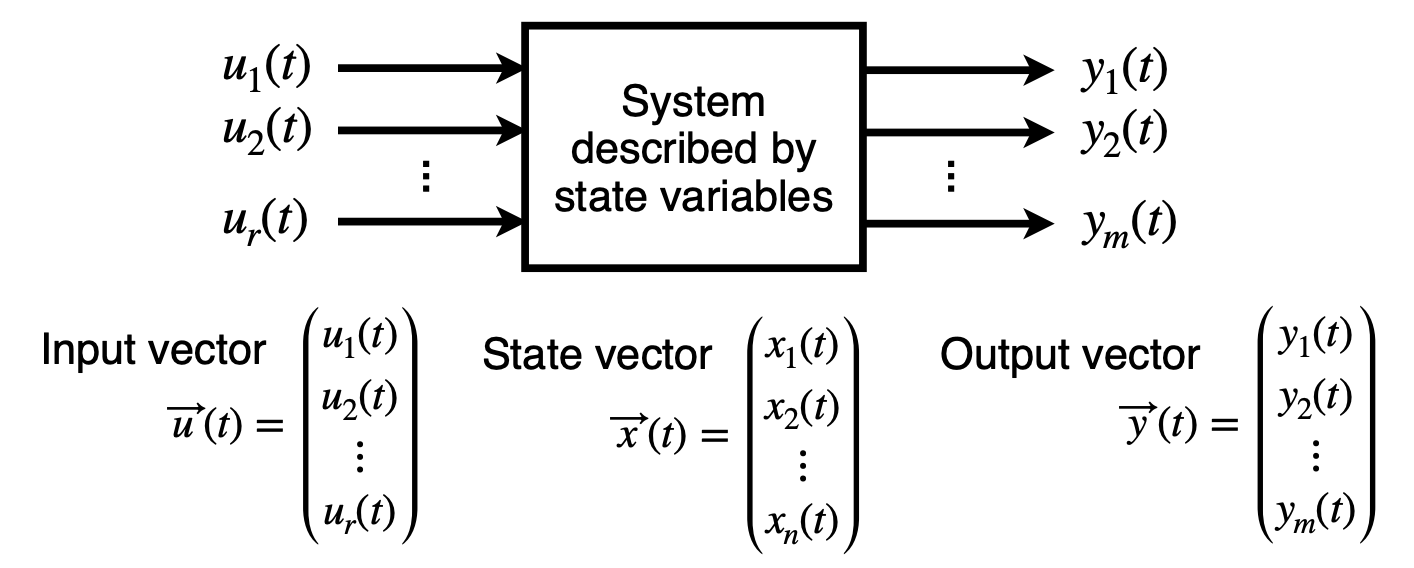
\includegraphics[width=0.65\textwidth]{images/multi_io.png}
        \caption{Multi-input/multi-output systems}
    \end{figure}

  \item The dynamics of state variables can be described by the 1$^{st}$ order differential equations, known as the \textbf{state equation}.
    \[\frac{d}{dt}\mathbf{x} = A\mathbf{x}+B\mathbf{u}\]
  \begin{itemize}
        \item $A$ is a $n\times n$ matrix, known as the \textbf{state matrix}, $ A \in \mathbb{R}^{n\times n}$.
        \item $B$ is a $n \times r$ matrix, known as the \textbf{input matrix}, $B \in \mathbb{R}^{n\times v}$.
  \end{itemize}
  
  \item \textbf{Output equation}: 
   \[\mathbf{y} = C\mathbf{x}+D\mathbf{u}\]
  \begin{itemize}
        \item $C$ is a $m\times n$ matrix, known as the \textbf{output matrix}, $ C \in \mathbb{R}^{m\times n}$.
        \item $D$ is a $m \times r$ matrix, known as the \textbf{feedthrough matrix}, $D \in \mathbb{R}^{m\times r}$.
  \end{itemize}
  
  \item \textbf{The transfer function} can be derived through taking the Laplace transform to the state-space model:
  \[G(s) = \frac{\mathbf{y}(s)}{\mathbf{u}(s)} = C(sI-A)^{-1}B+D\]
\end{itemize}
%---------------EXAMPLE START---------------%
\begin{ex}{}
\[G(s) = \frac{s+4}{s^{2}+3s+2} \quad \longleftrightarrow \quad (s^{2}+3s+2)Y(s) = (s+4)U(s)\]
This gives us a 2nd order O.D.E.
\[\ddot{y}+3\dot{y}+2y = \dot{u}+4u\]
\end{ex}
There are an infinite number of possible state-space models.
%----------------EXAMPLE END----------------%

%-------------------------------------------%
\subsection{Canonical Forms}
%-------------------------------------------%
Given a transfer function, there are infinite number of possible state-space representations.
\begin{itemize}
    \item A system is \textbf{controllable} if there exists an input that can move its state variable from an initial state to any arbitrary state in a finite time.
    
    \item A system is \textbf{observable} if its states at any time point can be determined by observing the output over a finite interval of time.
\end{itemize}

For the system:
\[ 
G(s) = \frac{Y(s)}{U(s)}=\frac{b_{1} s^{n-1}+b_{2} s^{n-2}+... +b_{n-1}s+b_{n}}{s^{n}+a_{1} s^{n-1}+...+a_{n-1}s+a_{n}} 
\]
\begin{itemize}
    \item The controllable canonical form is given by:
    \begin{gather*}
    \begin{pmatrix}
    \dot{x}_{1}\\
    \dot{x}_{2}\\
    \vdots\\
    \dot{x}_{n-1}\\
    \dot{x}_{n}
    \end{pmatrix} =
    \begin{pmatrix}
    0 & 1 & 0 & \ldots & 0\\
    0 & 0 & 1 & \ldots & 0 \\
    \vdots &\vdots &\vdots  & \ddots & \vdots \\
    0 & 0 & 0 & \ldots & 1\\
    -a_{n} & -a_{n-1} & -a_{n-2} & \ldots & -a_{1}
    \end{pmatrix} 
    \begin{pmatrix}
    {x}_{1}\\
    {x}_{2}\\
    \vdots\\
    {x}_{n-1}\\
    {x}_{n}
    \end{pmatrix}
    +
    \begin{pmatrix}
    0\\
    0\\
    \vdots\\
    0\\
    1
    \end{pmatrix}u
    \end{gather*}
    \begin{gather*}
    y = \begin{pmatrix}
    b_{n}&b_{n-1}&b_{n-1}&\ldots&b_{1}
    \end{pmatrix}
    \mathbf{x}
    \end{gather*}

%---------------EXAMPLE START---------------%
    \begin{ex}{}
    The system
    \[G(s) = \frac{s+4}{s^{2}+3s+2}\]
    can be written as (in controllable canonical form)
    \begin{gather*}
    \begin{pmatrix}
    \dot{x}_{1}\\
    \dot{x}_{2}\\
    \end{pmatrix} = 
    \begin{pmatrix}
    0&1\\
    -2&-3\\
    \end{pmatrix}
    \begin{pmatrix}
    x_{1}\\
    x_{2}\\
    \end{pmatrix}
    +
    \begin{pmatrix}
    0\\
    1\\
    \end{pmatrix}u
    \end{gather*}
    \begin{gather*}
    y = 
    \begin{pmatrix}
    4&1\\
    \end{pmatrix}
    \begin{pmatrix}
    x_{1}\\
    x_{2}\\
    \end{pmatrix}
    +0u
    \end{gather*}
    To verify this, start from the definition of the transfer function:
    \begin{equation*}
    \begin{aligned}
    G(s) &= \frac{\mathbf{y}(s)}{\mathbf{u}(s)} = C(sI-A)^{-1}B+D\\
    &= \begin{pmatrix}
     4 & 1\\
    \end{pmatrix}
    \{sI-\begin{pmatrix}
    0&1\\
    -2&-3\\
    \end{pmatrix}
    \}^{-1}
    \begin{pmatrix}
    0\\
    1\\
    \end{pmatrix}\\
    &=\begin{pmatrix}
     4 & 1\\
    \end{pmatrix}
    \begin{pmatrix}
    s&-1\\
    2&s+3\\
    \end{pmatrix}
    ^{-1}
    \begin{pmatrix}
    0\\
    1\\
    \end{pmatrix}\\
    &=\begin{pmatrix}
     4 & 1\\
    \end{pmatrix}
    \frac{1}{s(s+3)+2}
    \begin{pmatrix}
    s+3&1\\
    -2&s\\
    \end{pmatrix}
    \begin{pmatrix}
    0\\
    1\\
    \end{pmatrix}\\
    &= \frac{s+4}{s(s+3)+2}
    \end{aligned}
    \end{equation*}
    \end{ex}
%----------------EXAMPLE END---------------%


    \item The observable canonical form is given by:
    \begin{gather*}
    \begin{pmatrix}
    \dot{x}_{1}\\
    \dot{x}_{2}\\
    \vdots\\
    \dot{x}_{n-1}\\
    \dot{x}_{n}
    \end{pmatrix} =
    \begin{pmatrix}
    0 & 0 &  \ldots & 0& -a_{n}\\
    1 & 0 &  \ddots &  \vdots &  -a_{n-1}\\
    0 &1 &\ddots  & \vdots & \vdots \\
    \vdots & \ddots & \ddots & 0 & -a_{2}\\
    0 & \ldots & 0 & 1 & -a_{1}
    \end{pmatrix} 
    \begin{pmatrix}
    {x}_{1}\\
    {x}_{2}\\
    \vdots\\
    {x}_{n-1}\\
    {x}_{n}
    \end{pmatrix}
    +
    \begin{pmatrix}
    b_{n}\\
    b_{n-1}\\
    \vdots\\
    b_{2}\\
    b_{1}
    \end{pmatrix}u
    \end{gather*}
    \begin{gather*}
    y = \begin{pmatrix}
    0&0&\ldots&0&1\\
    \end{pmatrix}
    \mathbf{x}
    \end{gather*}

%---------------EXAMPLE START---------------%
    \begin{ex}{}
        The system 
        \[G(s) = \frac{s+4}{s^{2}+3s+2}\]
        can be written as  (in observable canonical form)
        \begin{gather*}
        \begin{pmatrix}
        \dot{x}_{1}\\
        \dot{x}_{2}\\
        \end{pmatrix} = 
        \begin{pmatrix}
        0&-2\\
        1&-3\\
        \end{pmatrix}
        \begin{pmatrix}
        x_{1}\\
        x_{2}\\
        \end{pmatrix}
        +
        \begin{pmatrix}
        4\\
        1\\
        \end{pmatrix}u
        \end{gather*}
        \begin{gather*}
        y = 
        \begin{pmatrix}
        0&1\\
        \end{pmatrix}
        \begin{pmatrix}
        x_{1}\\
        x_{2}\\
        \end{pmatrix}
        +0u
        \end{gather*}
        To verify this, start from the definition of the transfer function:
        \begin{equation*}
        \begin{aligned}
        G(s) &= \frac{\mathbf{y}(s)}{\mathbf{u}(s)} = C(sI-A)^{-1}B+D\\
        &= \begin{pmatrix}
         0 & 1\\
        \end{pmatrix}
        \{sI-\begin{pmatrix}
        0&-2\\
        1&-3\\
        \end{pmatrix}
        \}^{-1}
        \begin{pmatrix}
        4\\
        1\\
        \end{pmatrix}\\
        &=\begin{pmatrix}
         0 & 1\\
        \end{pmatrix}
        \begin{pmatrix}
        s&2\\
        -1&s+3\\
        \end{pmatrix}
        ^{-1}
        \begin{pmatrix}
        4\\
        1\\
        \end{pmatrix}\\
        &=\begin{pmatrix}
         0 & 1\\
        \end{pmatrix}
        \frac{1}{s(s+3)+2}
        \begin{pmatrix}
        s+3&-2\\
        1&s\\
        \end{pmatrix}
        \begin{pmatrix}
        4\\
        1\\
        \end{pmatrix}\\
        &= \frac{s+4}{s(s+3)+2}
        \end{aligned}
        \end{equation*}
    \end{ex}
%----------------EXAMPLE END----------------%
\end{itemize}


%-------------------------------------------%
\subsection{Stability of State-space Model}
%-------------------------------------------%
The system is stable if all eigenvalues of $A$ satisfies $\Re(\lambda_{i})<0$. \textit{i.e.} All eigenvalues of $A$ are on the left-side of the s-plane.\\\\
There are 2 ways to find the matrix exponential:
\begin{itemize}
    \item Diagonalisation of $A$;
    \item Using the identity: $e^{At} = \mathcal{L}^{-1}(sI-A)^{-1}$.
\end{itemize}


%-------------------------------------------%
\subsubsection{Solutions of State-space Model}
%-------------------------------------------%
\[\mathbf{x}(t) = \underbrace{e^{At}\mathbf{x}(0)}_{\text{zero-input response}}+\underbrace{\int_{0}^{t}e^{A(t-\tau)}B\mathbf{u}(\tau)d\tau}_{\text{zero-state response}}\]
\[\mathbf{y}(t) = Ce^{At}\mathbf{x}(0)+C\int_{0}^{t}e^{A(t-\tau)}B\mathbf{u}(\tau)d\tau+D\mathbf{u}(\tau)\]

%---------------EXAMPLE START---------------%
\begin{ex}{}
Find the response of the system where 
\begin{gather*}
\mathbf{\dot{x}}=\begin{pmatrix} -
2&0\\
1&-1
\end{pmatrix}
\mathbf{x}+
\begin{pmatrix}
1\\0
\end{pmatrix}u
\end{gather*}
and $\mathbf{x}(0)=\begin{pmatrix} 0\\0 \end{pmatrix}$, $u(t)=5$, $y =\begin{pmatrix}
2&1\\
\end{pmatrix}
 \mathbf{x}$
\vspace{.2cm}\hrule
\[\mathbf{x}(t) = e^{At}\mathbf{x}(0)+\int_{0}^{t}e^{A(t-\tau)}B\mathbf{u}(\tau)d\tau\]
Since\footnote{derivation see below}
\[e^{At} = \begin{pmatrix}
e^{-2t} & 0\\
e^{-t}-e^{-2t} & e^{-t}\\
\end{pmatrix}
\]
Therefore
\begin{equation*}
\begin{aligned}
\mathbf{x}(t) &= \begin{pmatrix}
e^{-2t} & 0\\
e^{-t}-e^{-2t} & e^{-t}\\
\end{pmatrix}
\int^{t}_{0}
\begin{pmatrix}
e^{-2\tau} & 0\\
e^{-\tau}-e^{2\tau} & e^{-\tau}
\end{pmatrix}
\begin{pmatrix}
5\\
0\\
\end{pmatrix}d\tau\\\\
&=\begin{pmatrix}
e^{-2t} & 0\\
e^{-t}-e^{-2t} & e^{-t}\\
\end{pmatrix}
\begin{pmatrix}
\int_{0}^{t} 5e^{2\tau}d\tau\\
\int_{0}^{t} (5e^{\tau}-5e^{2\tau})d\tau\\
\end{pmatrix}\\\\
&=\begin{pmatrix}
\frac{5}{2}(1-e^{-2t})\\
\frac{5}{2}(1+e^{-2t})-5e^{-t}
\end{pmatrix}
\end{aligned}
\end{equation*}

\begin{gather*}
y = (2 \ 1)\mathbf{x} = (2 \ 1)\begin{pmatrix}
\frac{5}{2}(1-e^{-2t})\\
\frac{5}{2}(1+e^{-2t})-5e^{-t}
\end{pmatrix}
 = \frac{15}{2}-\frac{5}{2}e^{-2t}-5e^{-t}
\end{gather*}

\vspace{.3cm}\hrule\vspace{.3cm}
Matrix exponential: $e^{tA} = Ve^{tD}V^{-1}$
\[tA = V(tD)V^{-1}\]
When eigenvalues of $A$ are $\lambda_{1}$, $\lambda_{2}$, ...Eigenvalues of $tA$ are $t\lambda_{1}$, $t\lambda_{2}$, ...
\[e^{tA} = \sum^{\infty}_{k=0}\frac{(tA)^{k}}{k!} =\sum^{\infty}_{k=0}\frac{V(tA)^{k}V^{-1}}{k!} = V\bigg(\sum^{\infty}_{k=0}\frac{(tA)^{k}}{k!}\bigg)V^{-1} \]

\begin{equation*}
\begin{aligned}
\sum^{\infty}_{k=0}\frac{(tA)^{k}}{k!}  &=\sum^{\infty}_{k=0}\frac{1}{k!} \begin{pmatrix}
(t\lambda_{1})^{k}&0&\ldots&0\\
0&(t\lambda_{2})^{k}&\ldots&0\\
\vdots&\vdots&\ddots&\vdots\\
0&0&\ldots&(t\lambda_{n})^{k}
\end{pmatrix}\\\\
&=\begin{pmatrix}
\sum^{\infty}_{k=0}\frac{(t\lambda_{1})^{k}}{k!} &0&\ldots&0\\
0& \sum^{\infty}_{k=0}\frac{(t\lambda_{2})^{k}}{k!}&\ldots&0\\
\vdots&\vdots&\ddots&\vdots\\
0&0&\ldots&\sum^{\infty}_{k=0}\frac{(t\lambda_{n})^{k}}{k!}
\end{pmatrix}\\\\
&=\begin{pmatrix}
e^{t\lambda_{1}}&0&\ldots&0\\
0&e^{t\lambda_{2}}&\ldots&0\\
\vdots&\vdots&\ddots&\vdots\\
0&0&\ldots&e^{t\lambda_{n}}
\end{pmatrix}\\\\
&= e^{tD}
\end{aligned}
\end{equation*}
\end{ex}
%----------------EXAMPLE END----------------%


%-------------------------------------------%
\subsubsection{Impulse Response}
%-------------------------------------------%
Transfer function\[G(s) = \frac{\mathbf{y}(s)}{\mathbf{u}(s)}=C(sI-A)^{-1}B+D\]
Impulse response\[\mathbf{y}(t) = Ce^{At}B+D\]
\begin{equation*}
\begin{split}
    \frac{d}{dt}e^{At} = Ae^{At} \xrightarrow{\mathcal{L}} & s\mathcal{L}(e^{At})-e^{A0} = A\mathcal{L}(e^{At})\\
    &(sI-A)\mathcal{L}(e^{At}) = e^{A0} = I\\
    &\mathcal{L}(e^{At}) = (sI-A)^{-1}\\
    &e^{At} = \mathcal{L}^{-1}(sI-A)^{-1}\\
\end{split}
\end{equation*}

%-------------------------------------------%
\subsubsection{Stability of State-space Models}
%-------------------------------------------%
\begin{align*}
\begin{split}
    G(s) &= C(sI-A)^{-1}B+D \\
    &=C\frac{1}{det(sI-A)}(sI-A)^{T}_{cofactor}B+D
\end{split}
\end{align*}
Poles $s$ of $G(s)$ = Eigenvalues $\lambda$ of $A$.
\[det(sI-A) = det(\lambda I-A) = 0\]
System is stable \textit{if and only if} $\Re (\lambda_{i})<0$ for all eigenvalues $\lambda_{i}$ of $A$.
 
 
%-------------------------------------------%
\subsubsection{Pole Placement}
%-------------------------------------------%
\begin{itemize}
\item \textbf{SISO system}: Poles of the closed-loop system as a function of the gain $K$: $\displaystyle \frac{Y(s)}{R(s)} = \frac{G(s)}{1+KG(s)}$.
\begin{figure}[H] 
    \centering
    % 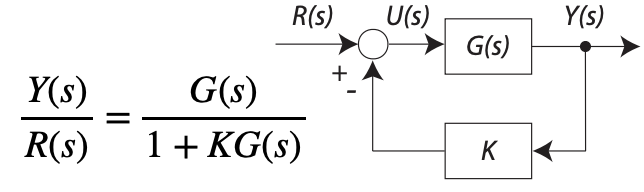
\includegraphics[width=0.4\textwidth]{images/SISO.png}
    \begin{tikzpicture}[auto, node distance=2cm,>=latex', line width = 1pt]
    \node [input, name=input] {};
    \node [sum, right of=input] (sum) {};
    \node [block, right of=sum] (controller1) {$G(s)$};
    \node [block, below= 0.5cm of controller1] (controller2) {$K$};
    \coordinate [right=1cm of controller1, circle, scale=0.5, fill](tooutput){};
    \node [output, right=1cm of tooutput] (output) {};

    \draw [draw,->] (input) -- node {$R(s)$\ {\footnotesize$+$}} (sum); 
    \draw [->] (sum) -- node {$U(s)$} (controller1);
    \draw [-] (controller1) -- (tooutput);
    \draw [-] (controller1) -- (tooutput) |- (controller2) ;
    \draw [->] (controller2) -| node[pos=1] {{\footnotesize$-$}} (sum);
    \draw [->] (tooutput) -- node[] {$Y(s)$} (output);
\end{tikzpicture}
    \caption{SISO system}
\end{figure}
\item \textbf{MIMO system}: 
\[\dot{x} = Ax+Bu = Ax +B(r-Kx) = (A-BK)x+Br\]
Eigenvalues of the matrix $(A-BK)$ determines the closed-loop stability.

\begin{figure}[H] 
    \centering
    % 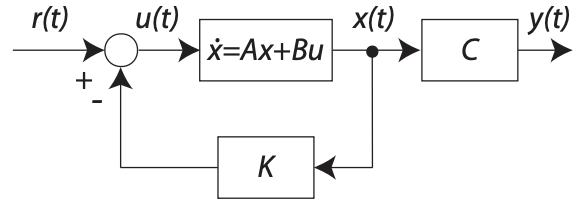
\includegraphics[width=0.4\textwidth]{images/MIMO.png}
    \begin{tikzpicture}[auto, node distance=2cm,>=latex', line width=1pt]
    \node [input, name=input] {};
    \node [sum, right of=input] (sum) {};
    \node [block, right= 1cm of sum] (controller1) {$\dot{x}=Ax+Bu$};
    \node [block, below= 1cm of controller1] (controller2) {$K$};
    \node [right=1cm of controller1, circle, fill, scale=0.5](tocon3){};
    \node [block, right= 1cm of tocon3] (controller3) {$C$};
    \node [output, right=1cm of controller3] (output) {};

    \draw [draw,->] (input) -- node {$r(t)$\ {\footnotesize$+$}} (sum); 
    \draw [->] (sum) -- node {$u(t)$} (controller1);
    \draw [-] (controller1) -- (tocon3)node[above = .1cm]{$x(t)$};
    \draw [->] (tocon3) -- node {} (controller3) -- node[]{$y(t)$}(output);
    
    \draw [->](tocon3) |- (controller2) -| node[pos=1] {{\footnotesize$-$}} (sum);
\end{tikzpicture}
    \caption{MIMO system}
\end{figure}
\end{itemize}
%---------------EXAMPLE START---------------%
\begin{ex}{}
\begin{equation*}
\begin{pmatrix}
\dot{x}_{1}\\
\dot{x}_{2}\\
\end{pmatrix} = 
\begin{pmatrix}
-0.5&-0.8\\
0.8&0\\
\end{pmatrix}
\begin{pmatrix}
x_{1}\\
x_{2}\\
\end{pmatrix}
+\begin{pmatrix}
1\\
0\\
\end{pmatrix}
u
\end{equation*}
Poles at $-0.25\pm 0.76\mathbf{j}$.\ \\
Design a state-feedback:
\begin{equation*}
\hat{u} = \begin{pmatrix}
k_{1} & k_{2}\\
\end{pmatrix}
\begin{pmatrix}
x_{1}\\
x_{2}\\
\end{pmatrix}
\end{equation*}
So that the closed-loop system has the poles at $-1$ and $-2$:
\begin{equation*}
A-BK = \begin{pmatrix}
-0.5&-0.8\\
0.8&0\\
\end{pmatrix}-
\begin{pmatrix}
1\\
0\\
\end{pmatrix}
\begin{pmatrix} 
k_{1}&k_{2}\\
\end{pmatrix}
 = 
 \begin{pmatrix}
 -0.5-k_{1}&-0.8-k_{2}\\
 0.8&0\\
 \end{pmatrix}
\end{equation*}
\begin{equation*}
det\{\lambda I-(A-BK)\} = \begin{vmatrix}
\lambda+0.5+k_{1} & 0.8+k_{2}\\
-0.8&\lambda\\
\end{vmatrix}
= (\lambda +1)(\lambda +2) 
\end{equation*}
\[ \lambda(\lambda + 0.5 + k_{1}) + 0.8(0.8 + k_{2}) = (\lambda +1)(\lambda +2) \]
This gives two solutions: $k_{1}=2.5$ and $k_{2}=1.7$
\end{ex}
%----------------EXAMPLE END----------------%


%-------------------------------------------%
\subsection{Decouple Interconnected Systems}
%-------------------------------------------%
\subsubsection{Relationship Between Equivalent Systems}
The system \[G(s)=\frac{1}{(s-1)(s-2)}\] can be written in
controllable canonical form:
\begin{gather*}
\begin{pmatrix}
\dot{x}_{1}\\
\dot{x}_{2}\\
\end{pmatrix}
= \underbrace{\begin{pmatrix}
0 & 1\\
-2 &3 \\
\end{pmatrix}}_{A_{1}}
\begin{pmatrix}
x_{1}\\
x_{2}\\
\end{pmatrix}
+\begin{pmatrix}
0\\
1\\
\end{pmatrix} u
\end{gather*}
and observable canonical form:
\begin{gather*}
\begin{pmatrix}
\dot{x}_{1}\\
\dot{x}_{2}\\
\end{pmatrix}
= \underbrace{\begin{pmatrix}
0 & -2\\
1 &3 \\
\end{pmatrix}}_{A_{2}}
\begin{pmatrix}
x_{1}\\
x_{2}\\
\end{pmatrix}
+\begin{pmatrix}
1\\
0\\
\end{pmatrix}
u
\end{gather*}
Since the two forms come from one transfer function, the system stability must be the same.
More importantly, $A$ matrix determine the stability of the system.\\\\
Relationship between $A_{1}$ and $A_{2}$:
\begin{gather*}
\begin{pmatrix}
-5 & 1\\
1 & 1 \\
\end{pmatrix}
\begin{pmatrix}
0 & 1\\
-2 &3 \\
\end{pmatrix}
=
\begin{pmatrix}
0 & -2\\
1 &3 \\
\end{pmatrix}
\begin{pmatrix}
-5 & 1\\
1 & 1 \\
\end{pmatrix}
\end{gather*}
\[TA_{1} = A_{2}T \quad \leftrightarrow \quad A_{1}=T^{-1}A_{2}T\]
Moreover,  both matrices $A_{1}$, $A_{2}$ has same eigenvalues at 1 and 2. So $A_{1}$, $A_{2}$ can be digonalized to the same matrix.
\[D = \begin{pmatrix}
1 & 0\\
0 & 2\\
\end{pmatrix}
\]
with the relation
\[A_{1}V_{1} = V_{1}D \quad \quad A_{2}V_{2} = V_{2}D\]

\subsubsection{Decoupling of Interconnected Systems (\textit{from Math 2})}
Decoupling of interconnected systems are done by matrix digonalization. 
\begin{figure}[H] \centering
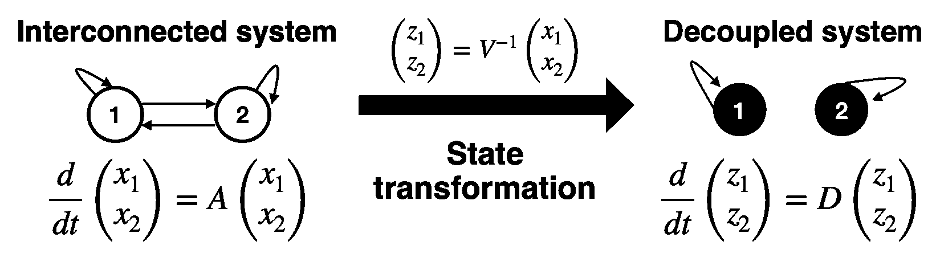
\includegraphics[width=.8\textwidth]{images/decouple.png}
\caption{De-couple an interconnected system}
\end{figure} \ \\
Decoupling of the interconnected system allows us to analyze the dynamics of a large system by only considering smaller systems.

%---------------EXAMPLE START---------------%
\begin{ex}{}
\begin{itemize}
\item Interconnected system:
\begin{equation*}
\frac{d}{dt} 
\begin{pmatrix}
x_{1}\\
x_{2}\\
\end{pmatrix}
=A
\begin{pmatrix}
x_{1}\\
x_{2}\\
\end{pmatrix}\quad \xrightarrow{A_{1}=\begin{pmatrix}
0 & 1\\
-2 & 3\\
\end{pmatrix}} \quad 
\begin{pmatrix}
\dot{x}_{1}\\
\dot{x}_{2}\\
\end{pmatrix} = 
\begin{pmatrix}
0 & 1\\
-2 & 3\\
\end{pmatrix}
\begin{pmatrix}
x_{1}\\
x_{2}\\
\end{pmatrix} = \begin{pmatrix}
x_{2}\\
-2x_{1}+3x_{2}\\
\end{pmatrix}
\end{equation*}

$\dot{x}_{1}$ and $\dot{x}_{2}$ depend on $x_{1}$ and $x_{2}$, this means the system is interconnected. 
\item Decoupled system:
\begin{equation*}
\frac{d}{dt} 
\begin{pmatrix}
z_{1}\\
z_{2}\\
\end{pmatrix}
=D
\begin{pmatrix}
z_{1}\\
z_{2}\\
\end{pmatrix} \quad \xrightarrow{D=\begin{pmatrix}
1 & 0\\
0 & 2\\
\end{pmatrix}} \quad 
\begin{pmatrix}
\dot{z}_{1}\\
\dot{z}_{2}\\
\end{pmatrix} = 
\begin{pmatrix}
1 & 0\\
0 & 2\\
\end{pmatrix}
\begin{pmatrix}
z_{1}\\
z_{2}\\
\end{pmatrix} = \begin{pmatrix}
z_{1}\\
2z_{2}\\
\end{pmatrix}
\end{equation*}
$\dot{z}_{1}$ only depends on $z_{1}$ and $\dot{z}_{2}$ only depends on $z_{2}$, this means the system is decoupled. 
\item The matrix D can be obtained by digonalization of matrix A
\[D =  V^{-1}AV\]
 \ where $V$ is the eigenvector.
\item The relationship between $z_{1}$, $z_{2}$ and $x_{1}$, $x_{2}$ satisfies:
\begin{gather*}
\begin{pmatrix}
z_{1}\\
z_{2}\\
\end{pmatrix}
=V^{-1}
\begin{pmatrix}
x_{1}\\
x_{2}\\
\end{pmatrix}
\end{gather*}
In this case:
\[V = \begin{pmatrix}
2&-1\\
-1&2\\
\end{pmatrix}\]
Therefore:
\begin{gather*}
\begin{pmatrix}
z_{1}\\
z_{2}\\
\end{pmatrix}
= 
\begin{pmatrix}
2&-1\\
-1&1\\
\end{pmatrix}
\begin{pmatrix}
x_{1}\\
x_{2}\\
\end{pmatrix}
\end{gather*}
\end{itemize}
\end{ex}
%----------------EXAMPLE END----------------%

%-------------------------------------------%
\subsection{Controllability and Observabiliy}
%-------------------------------------------%
\subsubsection{Controllability}
\begin{itemize}
    \item A system is controllable if there exists an input that can move its state variable from an initial state to any arbitrary state in a finite time;
    
    \item A systems is controllable if the controllability matrix is of full rank
    \[rank (B \ AB\ A^{2}B \ ...\ A^{n-1}B)=n\]
\end{itemize}

\subsubsection{Observability}
\begin{itemize}
    \item A system is observable if its states at any time point can be determined by observing the output over a finite interval of time.
    
    \item A system is observable if the observability matrix is of full rank.
\end{itemize}

\[rank \begin{pmatrix}
C       \\
CA      \\
CA^{2}  \\
\vdots  \\
CA^{n-1}
\end{pmatrix} 
= n
\]

\subsubsection{Stabilisability and Detectability}
\begin{itemize}
    \item A system is stabilisable if all the uncontrollable states are stable.
    
    \item A systems is detectable if all the unobservable states are stable.
\end{itemize}
